\documentclass[a4paper,UTF8,zihao=-4,scheme=chinese]{ctexbook}
\usepackage[backend=biber, maxbibnames=3, minbibnames=3, style=gb7714-2015,gbpub=false, gbnamefmt=lowercase,url=false]{biblatex} %% 文献处理宏包gbpub=false, 
\usepackage[Chinesetype=工学, Englishtype=Science, Chinesedegree=博士, Englishdegree=Doctor]{WUTthesis}
\usepackage[usenames, dvipsnames]{xcolor} %% 颜色宏包
\usepackage{setspace} %% 调整行距的宏包
\usepackage{graphicx} %% 和插图相关的宏包
\usepackage{xeCJKfntef}%%导入下划线%%原代码\WUTmakesecondcover报错
\usepackage{ifthen}%判断语句
\usepackage[colorlinks,linkcolor=black,anchorcolor=blue,citecolor=red,urlcolor=blue]{hyperref}  %设置超链接及其颜色,不想要参考文献引用有颜色的从这里修改
\usepackage{geometry}%设置页面大小
\usepackage{amssymb, amsfonts, amsmath, amsthm, mathtools} %% 和数学相关的一些宏包
\usepackage{float}%流动体宏包
\usepackage{setspace}%设置间距宏包
\usepackage{caption} %标题
\usepackage{booktabs}%画三线表用的
\usepackage{array} %% 制表宏包
\usepackage{multicol} %% 可以设置多列排版的宏包
\usepackage{multirow} %% 可以设置多行排版的宏包
\usepackage{enumerate} %%编号宏包
\usepackage{verbatim}%%批量注释宏包	\begin{comment} ... \end{comment}
\usepackage[linesnumbered,boxed,ruled,commentsnumbered,algochapter]{algorithm2e}%%算法包,注意设置所需可选项
\usepackage{longtable} %%长表格,可以分页显示的表格
\renewcommand{\algorithmcfname}{算法}

\captionsetup[table]{labelsep=space} % 引用表时冒号改为空格
\captionsetup[figure]{labelsep=space} % 图  

\raggedbottom %%顶部对齐
%% \parencite{Zhu2023} 中括号应用如文献[1]
\newcommand{\kuocite}[1]{\scalebox{1.3}[1.3]{\raisebox{-0.65ex}{#1}}} %%自定义函数用于大括号应用,如文献[1]不啦不啦。
\newcommand{\figref}[1]{图 \ref{#1} }
\newcommand{\tabref}[1]{表 \ref{#1} }


\renewcommand{\bibfont}{\zihao{5}} %% 设置参考文献字号五号

\renewcommand{\theequation}{\thechapter-\arabic{equation}} %% 将公式代号中默认的“.”改为“-”
\renewcommand{\thefigure}{\thechapter-\arabic{figure}} %% 将插图代号中默认的“.”改为“-”
\renewcommand{\thetable}{\thechapter-\arabic{table}} %% 将表格代号中默认的“.”改为“-”
\renewcommand{\thealgocf}{\thechapter-\arabic{algocf}} %% 将算法代号中默认的“.”改为“-”

\ctexset{chapter={format+={\zihao{-2}\heiti}, number={\arabic{chapter}}, beforeskip={6pt},afterskip={33pt},pagestyle={fancy},fixskip=true}} %% 设置章标题为字号小二,黑体,阿拉伯数字,章节标题与后面下方之间的距离为33pt
\CTEXsetup[format={\bfseries\raggedright}]{section}%%section标题左对齐
\ctexset{section={format+={\zihao{3}\heiti},afterskip={22pt}}} %% 设置节标题为字号三号,黑体,阿拉伯数字,章节标题与后面下方之间的距离为22pt
\ctexset{subsection={format+={\zihao{4}\heiti},afterskip={13.5pt}}} %% 设置二级节标题为字号四号,黑体,阿拉伯数字,章节标题与后面下方之间的距离为13.5pt
%\ctexset{subsubsection={format+={\zihao{-4}\heiti}, afterskip={7pt}}} %% 设置三级节标题为字号小四号,黑体,阿拉伯数字,章节标题与后面下方之间的距离为7pt
%\ctexset{paragraph/afterskip={6pt}}

\addbibresource{biber.bib} %% 加入参考文献书库库文件

\begin{document}


\WUTclassificationnumber{} %% 分类号
\WUTconfidentiality{} %% 密级:只有涉密论文才填写
\WUTUDC{} %% UDC
\WUTuniversitycode{10497} %% 学校代码

\WUTChinesetitle{锂离子电池电化学模型简化及其应用} %% 论文中文题目
\WUTEnglishtitle{Simplification and Applification of}{Electrochemical Models for Lithium-ion Betteries} %% 论文英文题目,由于一般英文题目过长,这里分成两行,所以这里相应地设置两个参数
\WUTauthor{孔纯}{Chun Kong} %% 论文作者:中文姓名,英文姓名
\WUTsupervisor{朱国荣}{Guorong Zhu}{教授}{博士}{武汉理工大学}{430000} %% 指导教师:中文姓名、英文姓名、职称、学位、单位名称、邮编
\WUTvicesupervisor{on}{某某某}{教授}{博士}{武汉理工大学}{430000} %% 副指导教师:on/off (是否有,没有就在封面不显示)、姓名、职称、学位、单位名称、邮编
\WUTmajor{交通信息工程及控制}{Traffic Information Engineering and Control} %% 二级学科:中文专业名称、英文专业名称
\WUTinstitute{自动化学院}{School of Automation} %% 院系名称
\WUTcommitteechairman{某某某} %% 答辩委员会主席
\WUTreviewers{某某某}{某某某}%% 评阅人
\WUTdegreeorganization{武汉理工大学} %% 学位授予单位
\WUTdates{2024年5月}{2024年5月}{2024年5月}{2024年6月}{May, 2024} %% 论文完成日期、论文完成日期、论文提交日期、论文答辩日期、学位授予日期、英文日期
\WUTdegreeabbreviation{Ph.D.} %% Ph.D. M.S. M.A.








\WUTmakefirstcover %% 生成封面一


\WUTmakesecondcover %% 生成封面二















\frontmatter %开始前面部分,从此页码为罗马数字
\let\cleardoublepage\clearpage %取消每章偶数页空白


\begin{titlepage}

\begin{adjustwidth}{6mm}{6mm}

\makebox[30mm]{\vspace{20mm}}

\begin{center}
\zihao{-2}\heiti 独创性声明
\end{center}
\vspace{5mm}
\begin{spacing}{1.4}
\par {\zihao{4}\STZhongsong  本人声明,所呈交的论文是本人在导师指导下进行的研究工作及取得的研究成果。尽我所知,除了文中特别加以标注和致谢的地方外,论文中不包含其他人已经发表或撰写过的研究成果,也不包含为获得武汉理工大学或其他教育机构的学位或证书而使用过的材料。与我一同工作的同志对本研究所做的任何贡献均已在论文中作了明确的说明并表示了谢意。}
\end{spacing}
\vspace{3mm}
\hspace{40mm}{\zihao{4}\STZhongsong 签\hspace{3mm}名:} \CJKunderline{\makebox[30mm]{}} \hspace{8mm} {\zihao{4}\STZhongsong 日\hspace{3mm}期:} \CJKunderline{\makebox[30mm]{}}


\vspace{40mm}




\begin{center}
\zihao{-2}\heiti 学位论文使用授权书
\end{center}
\vspace{3mm}
\begin{spacing}{1.4}
\par {\zihao{4}\STZhongsong 本人完全了解武汉理工大学有关保留、使用学位论文的规定,即学校有权保留并向国家有关部门或机构送交论文的复印件和电子版,允许论文被查阅和借阅。本人授权武汉理工大学可以将本学位论文的全部内容编入有关数据库进行检索,可以采用影印、缩印或其他复制手段保存或汇编本学位论文。同时授权经武汉理工大学认可的国家有关机构或论文数据库使用或收录本学位论文,并向社会公众提供信息服务。}
\end{spacing}
\vspace{3mm}
\hspace{53mm}{\zihao{4}\STZhongsong(保密的论文在解密后应遵守此规定)}

\vspace{20mm}
\noindent{\zihao{4}\STZhongsong 研究生(签名):} \hspace{20mm} {\zihao{4}\STZhongsong 导师(签名):} \hspace{20mm} {\zihao{4}\STZhongsong 日期:}


\end{adjustwidth}
\end{titlepage}





\setlength{\headwidth}{146mm} %设置页眉宽度
\newgeometry{left=3.2cm,right=3.2cm,top=3.5cm,bottom=3.5cm} %定义正文页间距

\begin{WUTChineseabstract}

%\sloppy
为减少大家写论文的排版工作量,让大家都能写出好看的,符合学校论文提交格式的论文。本人在顾加银同学做的{\LaTeX}论文模板\url{https://github.com/Jiayin-Gu/WUTthesis} 的基础上,根据武汉理工大学硕博论文格式要求做出了新的武汉理工大学硕博论文{\LaTeX}模板,网址为

\url{https://github.com/kon9chun/wutthesis2024}

大家可根据自己喜好选择使用哪种模板,也希望大家将该模板多多推广,早日让武汉理工大学官方接受{\LaTeX}排版论文。

本人使用MiKTeX编译工具,下载网址\url{https://miktex.org/}。习惯用其他的{\LaTeX}编译工具的同学请自行选择。

模板使用方式:先刷一遍XeLaTeX,再刷一遍biber,最后刷一遍XeLaTeX。

\end{WUTChineseabstract}
\WUTChinesekeywords{武汉理工大学,研究生,论文,{\LaTeX}模型}

\begin{WUTEnglishabstract}

English Abstract
\end{WUTEnglishabstract}
\WUTEnglishkeywords{Wuhan University of Technology, Postgraduates, Thesis, {\LaTeX} Template}




  %摘要


\tableofcontents %目录
% 插图目录,如不需要,删去
{%
\let\oldnumberline\numberline%
\renewcommand{\numberline}{\figurename~\oldnumberline}%
\listoffigures%
}

% 表格目录,如不需要,删去
{%
\let\oldnumberline\numberline%
\renewcommand{\numberline}{\tablename~\oldnumberline}%
\listoftables%
}

\chapter*{缩略词注释表}

% Table generated by Excel2LaTeX from sheet 'Sheet1'
\newcolumntype{L}[1]{>{\raggedright\arraybackslash}m{#1}}
\begin{spacing}{1.25}
\begin{longtable}[c]{lL{8cm}L{8em}}  % 
	\textbf{缩写} & \textbf{英文全称} & \textbf{中文全称} \vspace{6pt}\\
\endfirsthead
	\textbf{缩写} & \textbf{英文全称} & \textbf{中文全称} \vspace{6pt}\\
\endhead
\multicolumn{3}{r}{续下页}
\endfoot
\endlastfoot
        Adam & Adaptive moment & 自适应动量 \\ 
        BMS & Battery Management System & 电池管理系统 \\ 
        FOM & Fractional-order Model & 分数阶模型 \\ 
        FOMe & Fractional-order Model with Electrolyte & 考虑液相的分数阶模型 \\ 
        FOMeA & Fraction-order Model with Electrolyte considering Aging Mechanism & 考虑老化机理的FOMe \\ 
        FOMeS & Fraction-order Model with Electrolyte considering Stress & 考虑应力变化的FOMe \\ 
        FOMeT & Fractional-order Model with Electrolyte considering Thermal effect & 考虑温度影响的FOMe\\ 
        LrEM & Long Short-term Memory Networks with Residual Electrochemical Model & 基于带残差长短记忆神经网络的简化电化学模型 \\ 
        LSTM & Long Short-term Memory Networks & 长短记忆神经网络 \\ 
        LSTM\_Res & Long Short-term Memory Networks with Residual & 带残差项的长短记忆神经网络 \\ 
        MCMB & Mesophase Carbon Microbeags & 中间相碳微球 \\ 
        MSE & Mean Square Error & 均方误差 \\ 
        OCP & Open-circuit Potantial & 开路电势 \\ 
        OCV & Open-circuit Voltage & 开路电压 \\ 
        P2D & Pseudo 2-dimensional & 伪二维 \\ 
        PINN & Physics-informed Neural Networks & 物理信息神经网络 \\ 
        SEI & Solid Electrolyte Interphase & 固体电解质界面 \\ 
        SOC & State of Charge & 荷电状态 \\
        SOH & State of Health & 健康状态 \\ 
        SPMe & Single Particle Model with Electrolyte & 考虑液相的单颗粒模型 \\ 

\end{longtable}
\end{spacing}


  %缩略词表

\mainmatter %开启章节序号计数,重置页码,页码使用阿拉伯数字;
\chapter{这是第一章}

\section{第一章第一节}
这是第一章第一节

\subsection{第一章第一节第一小节}
毕业论文只允许使用三级标题,再要写字标题可以成编号的形式:
一个回车不换行

两个回车才换行。
\begin{enumerate}
\item 编号一
\item 编号二
\item 编号三
\end{enumerate}
还可以自定义编号的形式:
\begin{enumerate}[自定义1:]
\item 编号一
\item 编号二
\item 编号三
\end{enumerate}
\section{公式}
公式编写使用标准的{\LaTeX}公式语法,可以参考这个网址\url{https://www.latexlive.com/}。引用格式为:式(\ref{eq1-1}),式(\ref{eq1-4})
\begin{equation}
\left \{ \begin{aligned}
\dot U_1 &=  - {{{U_1}} \over {{R_1}{C_1}}} + {{{I_L}} \over {{C_1}}} \\
U_L &= {U_{oc}} - {U_1} - {I_L}{R_0}
\end{aligned}
\right.
\label{eq1-1}
\end{equation}

\begin{equation}
SOC= {Q_{pre} \over Q_{max}}\times 100\% \label{eq1-4}
\end{equation}

\section{图片}
插入图片显示如下,引用\figref{fig5-1},scale可以直接调整比例。[H]代表浮动体,删除则图片和表格自动调整,默认总是在页面最上方。
\begin{figure}[H]
\centering
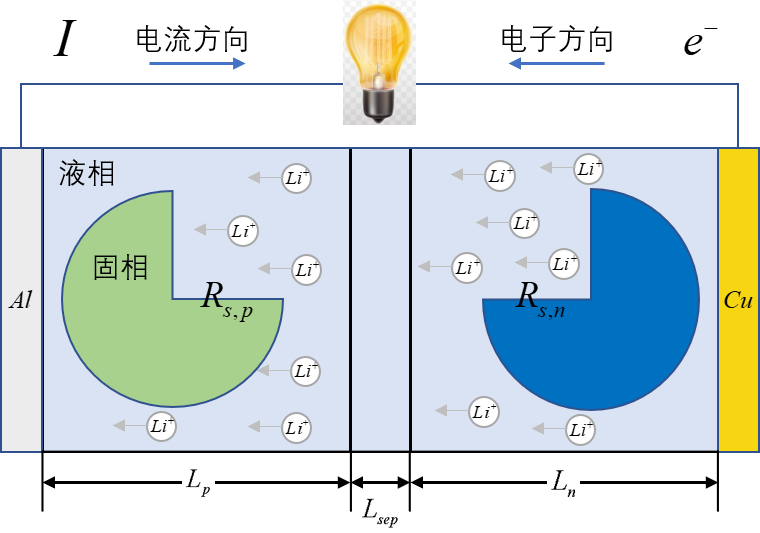
\includegraphics[scale=0.75]{figure/chap1/Li-ion.png}
\caption{FOMe原理示意图}
\label{fig5-1}
\end{figure}
也可设定长宽数值调整图片大小,如\figref{fig1-2}所示。
\begin{figure}[H]
\centering
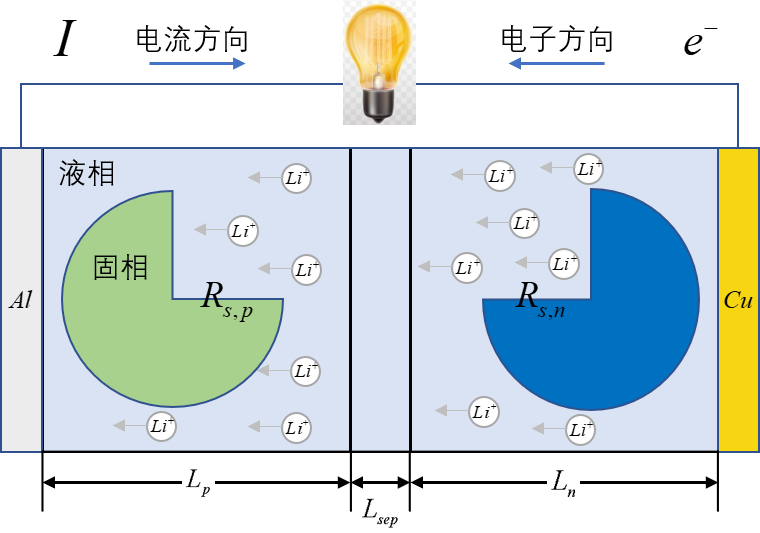
\includegraphics[width=6cm,height=6cm]{figure/chap1/Li-ion.png}
\caption{width=6cm,height=6cm}
\label{fig1-2}
\end{figure}

\section{表格}
表格使用方法如下,引用格式:如\tabref{tab1-1}
\begin{table}[H]%[htbp]
	\centering
	\begin{spacing}{1.35}
		\caption{锂离子电池、镍氢电池和铅酸电池性能对比}
		\label{tab1-1}
		\begin{tabular}{|m{2.5cm}<{\centering}|m{3.2cm}<{\centering}|m{3.2cm}<{\centering}|m{3.2cm}<{\centering}|}
			\hline
			特性  & 锂离子电池 & 镍氢电池 & 铅酸电池  \\%\tabincell{c}{阶乘数\\(十进制形式)} \\
			\hline
        工作电压(V) & 3.6 & 1.26 & 2 \\ \hline
        循环寿命(周次) & ≥800 & ≥500 & ≥300 \\ \hline
        自放电率(\%/月) & 5 & 20 & 30 \\ \hline
        环保性 & 不含重金属,相对传统电池更环保 & 含有重金属,不如镍氢电池和锂离子电池环保 & 不含重金属,相对于铅酸电池更环保 \\ \hline
		\end{tabular}
	\end{spacing}
\end{table}

三线表如\tabref{tab2-8}
\begin{table}[h!]
\centering
\begin{spacing}{1.35}
\caption{FOM,FOMe与P2D模型仿真耗时}
\label{tab2-8}
\begin{tabular}{cm{2.5cm}<{\centering}}
\toprule[1pt]
	电化学模型 	&	计算时间        \\
\midrule[0.5pt]
FOM &         0.3742s    \\
FOMe	&       0.3964s    \\
P2D   &   42s  \\
\bottomrule[1pt]
\end{tabular}
\end{spacing}
\end{table}

这个网址\url{https://tableconvert.com/zh-cn/excel-to-latex}提供了Excel表转{\LaTeX}格式的表。

\chapter{这是第二章}

\section{伪代码}
如需阐述算法看用伪代码形式展示,如算法 \ref{al2-2} 所示。

\begin{algorithm}[H]
    \SetAlgoNoLine % 不要算法中的竖线
    \SetKwInOut{Input}{\textbf{输入}}\SetKwInOut{Output}{\textbf{输出}} % 替换关键词
    \Input{
        \\
        当前电池开路电压OCV,FOM热力学参数;\\
}
    \Output{
        \\
        开路电压OCV对应的正负极初始嵌锂量;\\
}
    \BlankLine
    初始化正极嵌锂量$\theta_p$=0.5,正极嵌锂量范围[0, 1];\\ % 分号 \; 区分一行结束
    设置电压容差;\\
    \Repeat
        {仿真电压与开路电压之差小于预设容差}
        {计算电池总容锂量$Q_{Li}=\theta_p^0 \times Q_p+\theta_n^0 \times Q_n$;\\
        计算负极嵌锂量$\theta_n=(Q_{Li}-\theta_p \times Q_p)/Q_n$;\\
        预测电池电压$U=U_p(\theta_p)-U_n(\theta_n)$;\\
	  \eIf{$(OCV-U) \le 0$}{
        正极嵌锂上限$\theta_p^{max}=\theta_p$;}
        {正极嵌锂下限$\theta_p^{min}=\theta_p$;}	
        更新正极嵌锂量$\theta_p=(\theta_p^{max}+\theta_p^{min})/2$;\\
        }
    \caption{二分查找确定电极初始嵌锂量\label{al2-2}}
\end{algorithm}
\section{实用工具}
Ditto实用复制粘贴工具,直接在微软商店即可下载。
\begin{figure}[H]
\centering
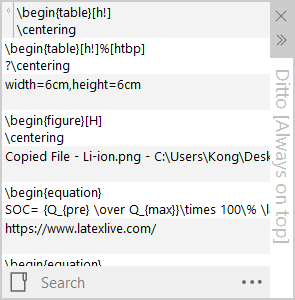
\includegraphics[scale=0.55]{figure/chap2/2-1.png}
\caption{Ditto}
\label{fig2-1}
\end{figure}
Jabref Bib文献工具,更方便的插入参考文献,网址地址\url{https://jabref.org/}。
\begin{figure}[H]
\centering
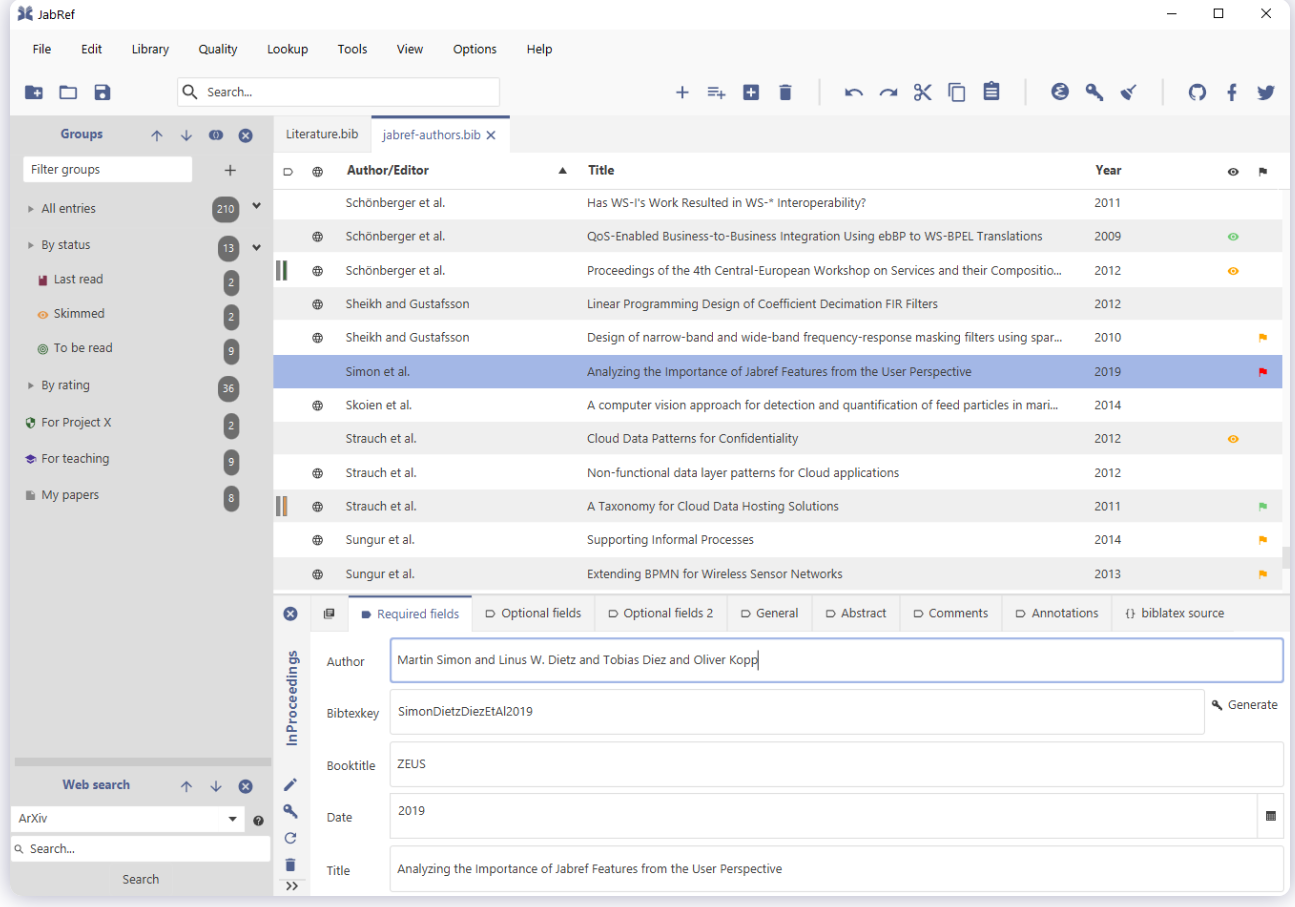
\includegraphics[scale=0.3]{figure/chap2/2-2.png}
\caption{Jabref}
\label{fig2-2}
\end{figure}
\section{参考文献引用}
上角标引用参考文献像这样\cite{Zhu2023},方括号引用,文献\parencite{Zhu2023a}不啦不啦不啦。更改了.bib文件要用biber刷一遍。


\backmatter %关闭章节序号,对页码没有影响;
\begin{WUTacknowledgements}
\par 致谢的字体为楷体小四,也可改为{\songti 宋体小四}。
\end{WUTacknowledgements}

%\begin{spacing}{1.3} %%可以适当调整spacing环境的参数,来控制参考文献的行距
\printbibliography[heading=bibintoc, title={参考文献}] %% 打印参考文献,采用了不同的颜色来区分各参考文献条目的内容
%\end{spacing}
\chapter{攻读学位期间获得与学位论文相关的科研成果}
\section*{学术论文}
\sloppy %{\zihao{5} 
\begin{enumerate}[ {[}1{]} ]
\item ZHU G, \textbf{KONG C}, WANG J V, et al. A fractional-order electrochemical lithium-ion batteries model considering electrolyte polarization and aging mechanism for state of health estimation[J]. Journal of Energy Storage, 2023, 72: 108649. DOI:10.1016/j.est.2023.108649. (SCI Q1, IF=9.4)
\item ZHU G, \textbf{KONG C}, WANG J V, et al. A fractional-order model of lithium-ion battery considering polarization in electrolyte and thermal effect[J]. Electrochimica Acta, 2023, 438: 141461. DOI:10.1016/j.electacta.2022.141461. (SCI Q1, IF=6.6)
\item ZHU G, \textbf{KONG C}, WANG J V, et al. A Simplified Electrochemical Lithium-ion Batteries Model based on Physics-informed Unsupervised Learning LSTM\_Res Network[J]. (已投”Journal of Power Source”在审)
\item ZHU G, \textbf{KONG C}, WANG J V, et al. A Simplified Electrochemical Model for Lithium-ion Batteries based on Ensemble Learning [J]. (已投”IScience”在审)
\item 朱国荣,\textbf{孔纯},王菁,等。锂离子电池电极颗粒破裂老化机理研究[J]。(电机工程学报在投)
\end{enumerate}
%}
\section*{专利}
















\end{document}